\section{Administración de Issues mediante GitHub CLI}

Posteriormente se realizó la administración de incidencias utilizando GitHub CLI desde la terminal Git Bash.

Como primer paso se verificaron los repositorios disponibles asociados a la cuenta autenticada mediante el siguiente comando:

\begin{lstlisting}
gh repo list
\end{lstlisting}

Este comando mostró los repositorios pertenecientes al usuario autenticado, permitiendo verificar el acceso a GitHub desde la terminal.

\begin{figure}[H]
\centering
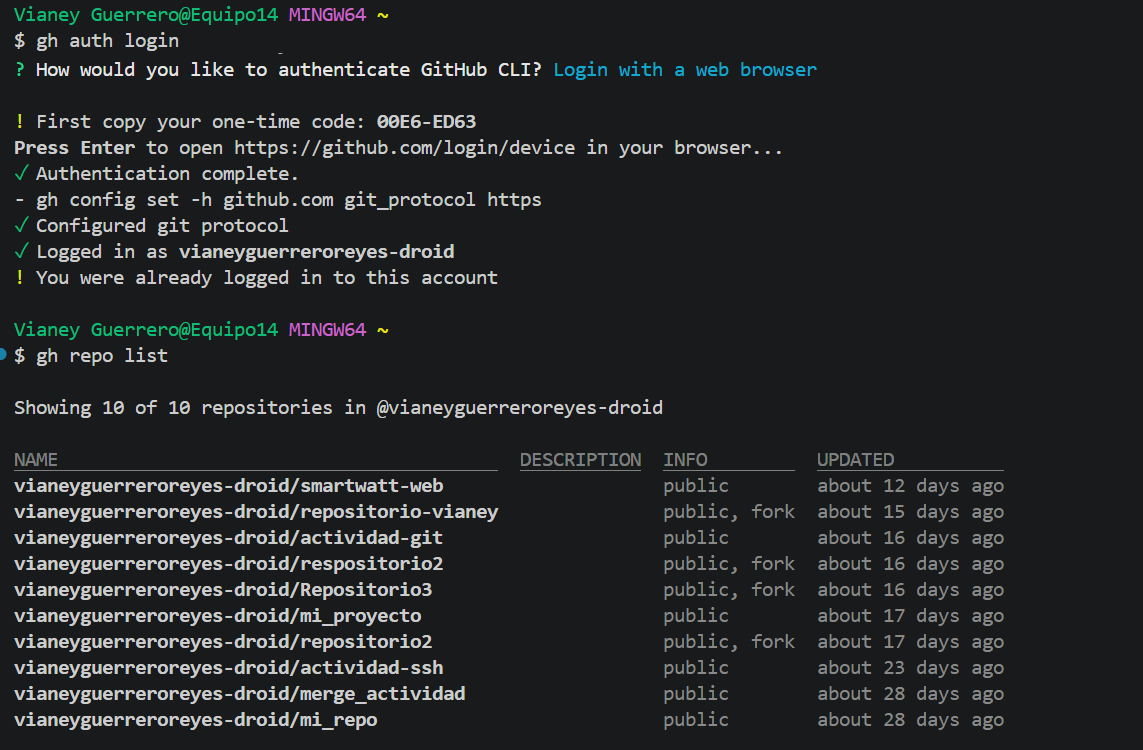
\includegraphics[width=0.9\textwidth]{M3.png}
\caption{Listado de repositorios disponibles mediante el comando gh repo list.}
\end{figure}

Debido a que el repositorio utilizado para la práctica pertenecía a otro integrante del equipo, fue necesario acceder directamente al repositorio mediante el siguiente comando:

\begin{lstlisting}
gh repo view martinezmoralesdiego2020-droid/repositorio
\end{lstlisting}

Con este comando se confirmó la existencia del repositorio y el acceso al mismo.

\begin{figure}[H]
\centering
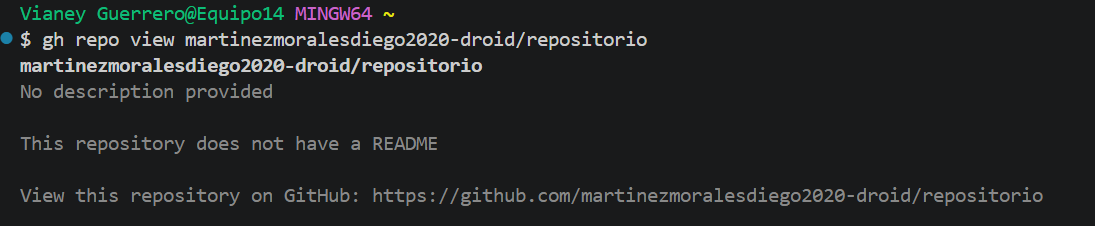
\includegraphics[width=0.9\textwidth]{M4.png}
\caption{Visualización del repositorio martinezmoralesdiego2020-droid/repositorio mediante GitHub CLI.}
\end{figure}

Posteriormente se consultaron los Issues existentes. En ese momento se observó que ya existían dos incidencias relacionadas con el problema de inicio de sesión.

\begin{figure}[H]
\centering
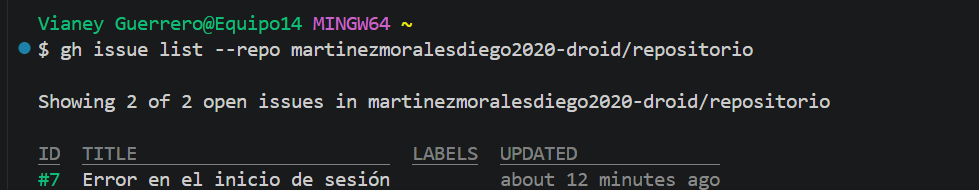
\includegraphics[width=0.9\textwidth]{M5.png}
\caption{Listado de Issues existentes en el repositorio.}
\end{figure}
